\subsection{Felépítés}
	A weboldal forráskódja a \texttt{/webpage} mappában helyezkedik el. 
	A fájlszerkezet az alábbi:
	\begin{figure}[h]
		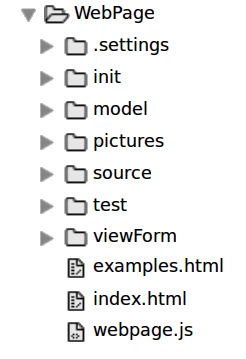
\includegraphics[width=4cm]{pics/folders_webpage}
		\centering
		\caption{A weboldal mappái\label{fig:folders_all}}
	\end{figure}
	\begin{description}
		\item[webpage.js :] \hfill \\  
		Globális változók inicializálása és pár alapbeállítás lefuttatása.
		
		\item[webpage.html :]  \hfill \\ 
		Weboldal megjelenítése, fájlok betöltése.
		
		\item[/init] \hfill \\ 
		Inicializáló függvények hívásai és események.
		\begin{description}
			\item[menulist.js : ] \hfill \\ 
				Interpolációk listájának inicializálója.
		  	\item[plot.js : ] \hfill \\ 
		  		Interpolációs grafikon inicializálása.
			\item[table.js : ] \hfill \\ 
				Interpolációs táblázat inicializálása.
		 	\item[events.js : ] \hfill \\ 
		 		Gombra kattintások eseményei.
		\end{description}

		\item[/model] \hfill \\ 
		Objektumok, melyeket az inicializáló lépésben hívunk, és azok segédletei.
		\begin{description}
		 	\item[base.js : ] \hfill \\
		 		Globális függvények \newline
		 		Base.get, Base.erlangJSON, Base.forEach.
		 	\item[base\_table.js : ] \hfill \\
		 		Általános táblázat generáló függvény.
		 	\item[connection.js : ] \hfill \\
		 		Szerver kapcsolat meghívására szolgáló függvény. \newline
		 		Connection.request
		 	\item[plot\_types.js : ] \hfill \\
		 		A grafikon kirajzoló típus objektumai.
		 	\item[polinome.js : ] \hfill \\  
		 		Polinom kirajzolását segítő függvények. \newline
		 		A makePolinome található benne és egyéb segédfüggvények.
		 	\item[web\_page\_debug.js : ] \hfill \\ 
		 		A Weboldalon történő kiíratást segítő objektum. \newline
		 		Jelenleg sehol nem használjuk már, de a megvalósítás során fontos szerepe volt a hibajavításban.
		\end{description}
		\item[/model/interpolation] \hfill \\
			Az oldal 3 fő részegységének függvényei:
			\begin{description}
			\item[menulist.js : ] \hfill \\ 
				Interpolációk lista megvalósítása. \newline
				function interpolationMenulist (aConfig) Objektum fájlja.
		  	\item[plot.js : ] \hfill \\ 
		  		Interpolációs grafikon megvalósítása. \newline
				function interpolationPlot(aConfig) Objektum fájlja.
			\item[table.js : ] \hfill \\
				Interpolációs táblázat megvalósítása. \newline
				function interpolationTable(aConfig) Objektum fájlja.
			\end{description}

		\item[/test] \hfill \\ 
			Olyan weboldal részlet fájlok, melyekből kialakult a mostani nagy fájl, és az objektumai, valamint tartalmaz még minta adathalmazokat.

		\item[/viewForm] \hfill \\ 
			Megjelenítéssel kapcsolatos css fájlokat tartalmazó mappa.
	\end{description}

\subsection{Fontosabb objektumok és függvények}
	\hfill
	Az objektumokat legtöbb esetben egy függvény generálja, melyeket a visszatérés után felhasználunk az eseménykezelésekhez.
	%%\ref{fig:webpage_big}
	%%\ref{fig:webpage_plot_class}
	%%\ref{fig:webpage_class_table}
	\begin{figure}[h]
		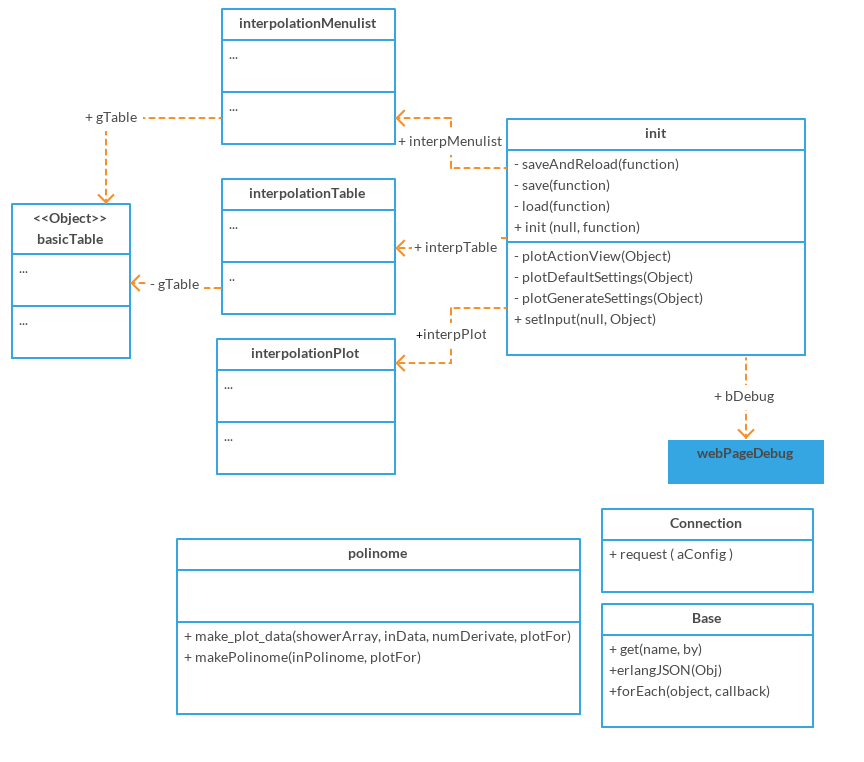
\includegraphics[width=14cm]{pics/webpage_big}
		\centering
		\caption{Weboldal osztálydiagramja\label{fig:webpage_big}}
	\end{figure}

	\begin{figure}[h]
		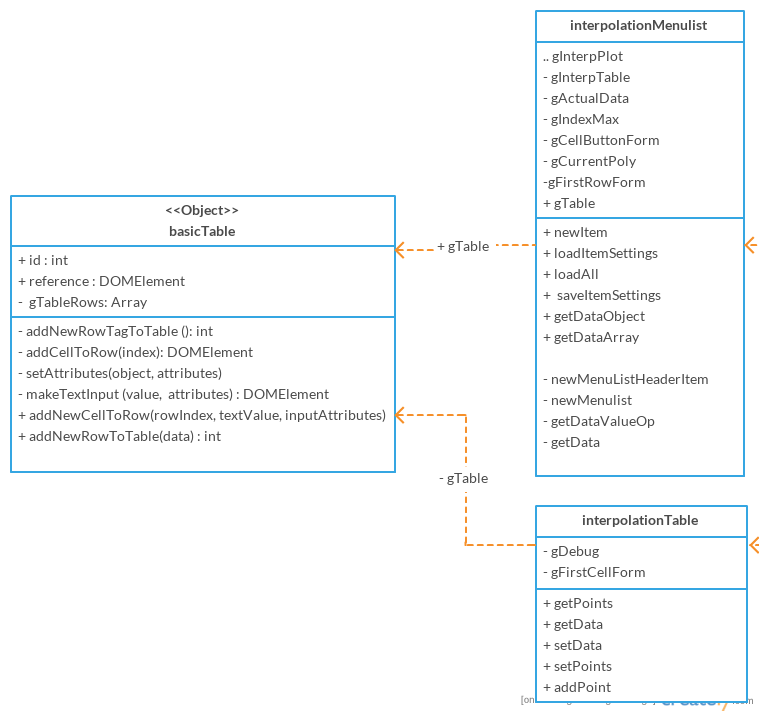
\includegraphics[width=14cm]{pics/webpage_class_table}
		\centering
		\caption{Táblázatok osztálydiagramja\label{fig:webpage_class_table}}
	\end{figure}

	\begin{figure}[h]
		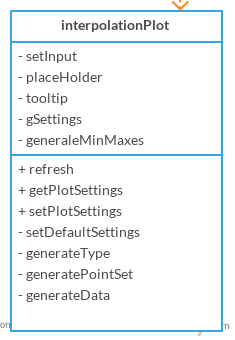
\includegraphics[width=5cm]{pics/webpage_plot_class}
		\centering
		\caption{Grafikon kirajzoló osztálydiagramja\label{fig:webpage_plot_class}}
	\end{figure}

	\begin{description}
		\item[makePolinome(inPolinome, plotFor)] \hfill \\ 
			Polinom pontjainak legenerálására szolgáló függvény, a grafikon kirajzolónak megfelelő típusban.
			\begin{description}
				\item[inPolinome] \hfill \\ 
					A polinom tömbös formában.
				\item[plotFor] \hfill \\ 
					A polinom intervalluma és pontossága.
			\end{description}
		\item[Connection.request(aConfig)] \hfill \\ 
			Elküldi a szervernek az értékeket.
			\begin{description}
				\item[aConfig.params] \hfill \\
				A kommunikációban a paraméter amelyet átküldünk a szervernek.
				\item[aConfig.callback] \hfill \\
				Sikeres visszatérés esetén ez a függvény fut le a szervertől vissza adott válasszal. 
			\end{description}
		\item[basicTable (aConfig)] \hfill \\ 
			Egy alap tábla objektum. Ennek segítségével lehet létrehozni az interpolációs táblázatot és a menü listát(interpoláció választó).
			\begin{description}
			\item[that.addNewCellToRow(rowIndex, textValue, inputAttributes)] 
				\hfill \\  Ad egy új cellát a sorhoz.
			\item[that.addNewRowToTable(data)]
				\hfill \\ Ad egy új sort a táblázathoz.
			\item[that.addNewColumnToTable(data)]
				\hfill \\ Ad egy új oszlopot a táblázathoz.
			\item[that.newTable()] 
				\hfill \\ Új tábla létrehozása.
			\item[that.setCellForm((i , j, attributes))] 
				\hfill \\ Egy adott cella megformázás beállítása.
			\item[that.getNumOfCols()] 
			 	\hfill \\ Visszatér az oszlopok számával.
			\item[that.getNumOfRows()]
				\hfill \\ Visszatér a sorok számával.
			\item[that.getRow(i)]
				\hfill \\ Visszatér a sor DOM-elemével az index alapján.\newline
				Ha nincs olyan indexű akkor null-al tér vissza.
			\item[that.getInputTag(i, j)]
				\hfill \\ Visszatér a tábla input elemével.
			\item[that.getValue(i, j)]
				\hfill \\ Egy adott cella érték lekérdezése.
			\item[that.findValue(column, value)] 
				\hfill \\ Megkeresi melyik sorban van egy adott értéket.
			\item[that.setValue(i, j, value, form)]
				\hfill \\ Beállít egy adott értéket egy cellának.
			\item[that.deleteTable()]
				\hfill \\ Teljesen törli a táblázatot.
			\item[that.remove(row)]
				\hfill \\ Kivesz egy sort a táblázatból.
			\item[addNewRowTagToTable ()]
				\hfill \\ Ad egy új sort a táblázathoz.
			\item[addCellToRow(index)]
				\hfill \\ Ad  egy cellát a sorhoz.
			\item[setAttributes(object, attributes)]
				\hfill \\ Beállítja egy objektum tulajdonságait.
			\item[makeTextInput (value,  attributes)]
				\hfill \\  
				TextInput hozzáadása a sorhoz.
			\end{description}
		\item[interpolationMenulist (aConfig)] 
			\hfill \\ 
			Az interpolációs menü függvénye. Itt tarjuk számon az aktuálisan betöltött adathalmazt.
			\begin{description}
			\item[that.newItem()] 
			\hfill \\ Új elemet vesz fel a listába. Gomb hatására is meghívódhat. \newline Új lista elem egy új interpolációs adathalmaz felvételét jelenti.  
			\item[that.getDataArray(server)] 
			\hfill \\ Visszatér az adathalmazzal, tömb formában. Ebben a formában küldjük fel a szervernek.
			\item[that.getDataObject()] 
			\hfill \\ Eredményül adja az adathalmazt, egy objektum formájában. Az Objektum értékeinek kulcsa, az interpolációk egyedi azonosítója (id-ja).
			\item[that.saveItemSettings()] 
			\hfill \\ Elmenti az adatokat az aktuálisan kijelölt sorba.
			\item[that.loadItemSettings(index)]
			\hfill \\ Feldogozza az adatsort a táblából, és betölti az adatokat a táblába.
			\item[that.loadAll(savedObject, resultObject)] 
			\hfill \\Betölti az összes Interpolációt az adott adathalmazból.
			\item[newMenulist()] 
			\hfill \\
			Új menülista: régi menü kitörlése, és egy új generálása.
			\hfill \\ 
			\end{description}
		\item[interpolationPlot (aConfig)]
			\hfill \\ Grafikon megjelenítése: \texttt{Flot} segítségével létrehoztam az alábbi Objektumot. Ebben valósítottam meg a kirajzolást, és annak tulajdonságait.
			\begin{description}
			\item[that.refresh(points, polynomials)]
			\hfill \\ Pontok és a polinomok alapján frissíti a grafikont.
			\item[that.getPlotSettings]
			\hfill \\ Visszatér a grafikon megjelenítési tulajdonságokkal. Ennek segítségével mentünk.
			\item[that.setPlotSettings]
			\hfill \\ Betölti a grafikon megjelenítési tulajdonságokat.
			\item[generateData(senderData, polynomial)]
			\hfill \\ Legenerálja a grafikon azon bemenő paraméterét, amely a megjelenítendő adatokat állítja.

			\item[generateType()]
			\hfill \\ Legenerálja a grafikon azon bemenő paraméterét, amely a grafikon megjelenítését állítja.
			\item[setDefaultSettings()]
			\hfill \\ Beállítja a grafikon paramétereit és értékeit az alapértelmezett értékekre.
			\item[generatePointSet(tableArray, derivNum)]
			\hfill \\ Legenerálja az adott pontokat, az interpolációs táblázatból.
			\end{description}

		\item[interpolationTable (aConfig)]
			\hfill \\ 
				Az interpolációs Táblázat logikája, és generálása. Ebben a táblázatban tekinthetjük meg a pontokat.
			\begin{description}
			\item[that.addPoint(x, y, dn)] 
			\hfill \\ Hozzá adja a pontot a táblázathoz. Ha létezik ezen az X-en pont akkor frissíti.
			\item[that.setPoints(tableArray)] 
			\hfill \\ Feltölti a táblázatot egy adott tömb értékeivel.
			\item[that.setData(data)] 
			\hfill \\ Feltölti az adatokkal a táblát.
			\item[that.getData()] 
			\hfill \\ Visszatér a táblázatban szereplő adatokkal.
			\item[that.getPoints()] 
			\hfill \\ Visszatér a táblázatban szereplő pontokkal.
			\end{description}
	\end{description}